\documentclass[10pt]{article}

% packages
\usepackage{verbatim}
\usepackage{amsmath}
\usepackage{amssymb}
\usepackage{amsthm}
\usepackage{array}
\usepackage{xy}
\usepackage{geometry}
\usepackage{enumitem}
\setlist{nolistsep}


% page formatting
\pdfpagewidth 8.5in
\pdfpageheight 11in
\oddsidemargin -.25in
\textwidth 6.75in
\textheight 9in
\topmargin -1.75in
\headheight 112pt
 
\usepackage[pdftex]{graphicx}
\usepackage{asymptote}
\usepackage{fancyhdr}
 
\pagestyle{fancy}
\fancyhf{}

 
 
 

% Header with logo
\lhead{\includegraphics{EPHeaderleft.png}}
\rhead{\includegraphics{EPHeaderright.png}}
% Footer
\cfoot{Copyright $\copyright$ 2012-16\hskip0.044in -- \hskip0.044in {\scalebox{.354} {\includegraphics{EPFooter.png}}}} 


\linespread{1.15}
\begin{document}



\setlength{\abovedisplayskip}{-10.2pt}
\setlength{\belowdisplayskip}{6.8pt}
\setlength{\abovedisplayshortskip}{0pt}
\setlength{\belowdisplayshortskip}{0pt}



\renewcommand{\labelitemi}{$\bullet$ \hskip0.04in}
\renewcommand{\labelitemii}{$\cdot$}
\renewcommand{\labelitemiii}{--}
\renewcommand{\labelitemiv}{$\ast$}


\centerline{\huge{2016 EP MC C Handouts}}

\clearpage

\centerline{\Large{Eat Pie Curriculum Pledge}} \vskip.1in

\centerline{\textbf{\noindent Please return by Monday, June 8, 2015.}}  \vskip0.33in

\noindent \emph{In order to maintain the intellectual integrity of the Eat Pie interns and instructors, I pledge that I will not share or distribute any classroom handouts, notes, materials, or problems sheets from $e\alpha\tau\cdot\pi ie$, with anybody. This includes friends, parents of friends, math team coaches, teachers, or other students at school who might ask for them.}

\vskip.5in
\centerline{\underline{\hskip6.5in}}\vskip.1in
\centerline{\underline{\hskip6.5in}}\vskip.1in
\centerline{\underline{\hskip6.5in}} \vskip0.1in
\centerline{\underline{\hskip6.5in}}\vskip.7in



Your signature: \underline{\hskip2in} \hskip1.8in Your name:\\ \\
\indent Signature of Agreeing Parent: \underline{\hskip2in}
\vskip.5in



\dotfill\\ \\ \\ 
\centerline{Congratulations! From now on, you will be under an honor code that you will not share any $e\alpha\tau\cdot\pi ie$}
\centerline{materials, problem sheets, or note handouts with anyone or the parties mentioned above.}
\\ \\
\centerline{If any parents, students, or math team teachers ask you to look at Eat Pie's materials, please direct them}
\centerline{to instructor.eatpie@gmail.com. Thank you for your cooperation.}
\\ \\ \\ \\ 
\centerline{\underline{\hskip2in}}
\centerline{The Eat Pie Team}


\vskip.7in

\clearpage

\centerline{\textbf{\Large{Advanced B in Review!}}}
\vskip0.1in
\centerline{``The Grad Pack'': Topics \& Examples}
\vskip0.5in

\begin{itemize}


\item \textbf{Principle of Inclusion-Exclusion (PIE)}:
\vskip0.1in
\begin{itemize}
% 15
\item In Nowhere Middle School, there are 74 students. 23 students take Algebra, 31 take Geometry, and 40 take Advanced Fiberglass Sculpting. If 18 take Algebra and Geometry, 21 take Geometry and Sculpting, and 4 are taking all three classes, how many people are taking Algebra and Sculpting?
\end{itemize}
\vskip0.6in


\item \textbf{Internal/External Tangents}
\vskip0.1in
\begin{itemize}

% 9, \sqrt{221}
\item Find the length of the internal and external tangents to two circles with radii 5 and 7, given that the distance between their centers is 15.

\end{itemize}
\vskip0.6in

\item \textbf{Stars and Bars}
\vskip0.1in
\begin{itemize}
% 28
\item Aditi is selecting six bags of chips from a box containing only Lays, Doritos, and Fritos. If there are at least six of each brand in the box, how many different chip assortments can she select?
\vskip0.1in
% 1716
\item Compute the number of distinct ways in which 77 one-dollar bills can be distributed to 7 people so that no person receives less than $\$ 10$ (ARML)
\end{itemize}
\vskip0.6in

\item \textbf{D=RT}
\vskip0.1in
\begin{itemize}
% 8
\item While Steve and LeRoy are fishing 1 mile from shore, their boat springs a leak, and water comes in at a constant rate of 10 gallons per minute. The boats will sink if it takes in more than 30 gallons of water. Steve starts rowing toward the shore at a constant rate of 4 miles per hour while LeRoy bails water out of the boat. What is the slowest rate, in gallons per minute, at which LeRoy can bail if they are to reach the shore without sinking? (AMC 10)

\end{itemize}
\vskip0.6in

\item \textbf{Modular Arithmetic}
\vskip0.1in

\begin{itemize}
%
\item The first day of the twenty first century, January 1, 2001, was a Monday. What day of the week will the first day of the twenty-second century be?
\vskip0.1in
% 6
\item Find $a$ where $0\le a\le 7$ and $11\cdot 18\cdot 2322\cdot 13\cdot 19\equiv a \pmod{7}$
\end{itemize}

\vskip0.6in
\item \textbf{Pathwalking}
\vskip0.1in
\begin{itemize}
% 210
\item A tiny, little, minuscule version of Godzilla wants to get from the point $(1,2)$ to $(6,9)$, but must pass through $(3,7)$ on the way. How any ways are there for him to do so?
\end{itemize}

\vskip0.6in
\item \textbf{3-D Geometry}
\vskip0.1in
\begin{itemize}
% 8/3
\item A regular tetrahedron is formed by connecting four out of the six vertices in a cube. Given that the side length of the cube is 2, what is the volume of the tetrahedron? Leave your answer in simplest radical form.
\end{itemize}
\vskip0.6in
\item \textbf{Algebraic Probability}
\vskip0.1in
\begin{itemize}
% 6/7
\item In 2010, the probability of Mark sinking a free throw was twice what it was in 2009, and yet the probability of him sinking exactly two out of three free throws was the same in both years. What was the probability of Mark sinking a free throw in 2010, given that the probability was greater than zero? Express your answer as a common fraction. (2011 National Sprint)
\end{itemize}
\vskip0.6in

\item \textbf{Geometric Probability}

\vskip0.1in
\begin{itemize}
% 1/8
\item A point $(x,y)$ is randomly picked from inside the rectangle vertices $(0,0)$, $(4,0)$, $(4,1)$, and $(0,1)$. What is the probability that $x<y$? (AMC 10)
\end{itemize}
\vskip0.6in


\item \textbf{Vieta's}

\vskip0.1in
\begin{itemize}
% -1
\item What is the sum of the reciprocals of the roots of the equation $\frac{2003}{2004}x+1+\frac{1}{x}=0$? (2003 AMC 10A)
\end{itemize}
\vskip0.6in


\item \textbf{Symmetric Equations}

\vskip0.1in
\begin{itemize}

% 5/2
\item Two positive numbers have the property that the sum of their squares is 20 and the sum of their reciprocals is 2. What is their product? Express your answer as a common fraction. (2012 State Sprint)
\vskip0.1in

% 65/8
\item If \scalebox{1.2}{$x+\frac{1}{x}=\frac{5}{2}$}, find \scalebox{1.2}{$x^3+\frac{1}{x^3}$}.
\end{itemize}
\vskip0.6in

\end{itemize}



\clearpage

\centerline{\textbf{\Large{Simon's Favorite Factoring Trick}}} \vskip0.1in
\centerline{\textit{SFFT for short}}

\vskip0.33in

\begin{itemize}

\item \textbf{Tipoffs}

\vskip0.17in

\begin{itemize}
\item You have a nasty $xy$ term
\item You're solving something in integers
\end{itemize}

\vskip0.17in

\item \textbf{How it works}

\vskip0.17in

\begin{itemize}
\item Think completing the square
\item Add some constant term to make everything factor
\item Typically we start with something like $xy+3x+5y$ and end with something like $(x+5)(y+3)-15$
\end{itemize}

\vskip0.33in

\item\textbf{Find all ordered pairs of integers $(x,y)$ such that $xy+4x+3y=5$.}
\vskip0.1in

We want to make the LHS look like $(x+?)(y+?)$. 

By expanding this, we see that the first ? should be 3 and the second ? should be 4.

But then to make this work, we are missing a $3\times 4$ term so we add 12 to the original equation.

\begin{align*}
xy+4x+3y+12 &= 5+12 \\
(x+3)(y+4) &= 17
\end{align*}

Now we use the fact that $x$ and $y$ must be integers, so we can make a chart.

\begin{center}
\begin{tabular}[t]{|c|c|c|c|}
\hline
$x+3$& $y+4$&$x$&$y$\\\hline\hline
1&17&-2&13\\\hline
17&1&14&-3\\\hline
-1&-17&-4&-21\\\hline
-17&-1&-20&-5\\\hline
\end{tabular}
\end{center}
\vskip0.1in
Finally, our solutions must be $(-2, 13)$, $(14, -3)$, $(-4, -21)$, and $(-20, -5)$.


\vskip0.33in


\item\textbf{Appetizers}

\begin{enumerate}
\vskip0.17in

\item Add a term to factorize the following expressions

\begin{itemize}

% +2
\item $ab+3a+5b+13$

% +7
\item $xy-2y+5x-17$

%
\item $2xy+4x-5y+23$

%
\item $3xy+2y-4x+13$

\end{itemize}

\vskip0.17in


% 2
\item How many rectangles with side lengths $x$, $y$ with $x\le y$ have equal perimeter and area?


\end{enumerate}

\end{itemize}

\clearpage


\centerline{\textbf{\Large{SFFT Problems}}} \vskip0.1in

\vskip0.33in

\begin{enumerate}

% 6
\item How many pairs of integers $(x,y)$ satisfy the equation $y=\frac{x+12}{2x-1}$ ? (AoPS)
\vskip0.26in

% 5
\item In how many different ways can $\frac{2}{15}$ be represented as $\frac{1}{a}+\frac{1}{b}$, if $a$ and $b$ are positive integers with $a\ge b$? (2005 State Team)

\vskip0.26in


% 56
\item For positive integers $n$ and $m$, each exterior angle of a regular $n$-sided polygon is 45 degrees larger than each exterior angle of a regular $m$-sided polygon. One example is $n=4$ and $m=8$ because the measures of each exterior angle of a square and a regular octagon are 90 degrees and 45 degrees, respectively. What is the greatest of all possible values of $m$? (2015 Chapter Sprint)
\vskip0.26in

% 15
\item How many pairs of natural numbers $(x,y)$ exist such that $\frac{1}{x}+\frac{1}{y}=\frac{1}{12}$? (2015 VHHS Comprehensive)
\vskip0.26in


% 1
\item Consider the set of all fractions $\frac{x}{y}$ where $x$ and $y$ are relatively prime positive integers. How many of these fractions have the property that if both numerator and denominator are increased by 1, the value of the fraction is increased by $10\%$? (2015 AMC 10A)
\vskip0.26in

% 588
\item Find $3x^2y^2$ if $x$ and $y$ are integers such that $y^2+3x^2y^2=30x^2+517$. (1987 AIME)
\vskip0.26in




\end{enumerate}



\clearpage

\centerline{\textbf{\Large{Intro to Sequences $\&$ Series:}}} 
\vskip0.33in

\begin{itemize}

\item \textbf{Arithmetic Sequence:} \hskip0.1in An ordered set of terms such that the difference between consecutive terms is a constant; often written: $a, a+r, a+2r,\dots$
\vskip0.17in

\item \textbf{Geometric Sequence:} \hskip0.1in An ordered set of terms in which each term after the first is formed by multiplying the previous term by a nonzero constant, called the constant ratio;  often written: $a, ar, ar^2, ar^3,\dots$
\vskip0.17in

\centerline{\emph{So what is a ``series"?}}
\centerline{\textbf{Series:} The sum of all the terms in a given sequence}
\vskip0.3in



\item \textbf{Arithmetic Series}
\vskip0.11in



\begin{enumerate}[label=\textbf{\Alph*.}]
\setlength{\itemindent}{2em}
\item \hskip0.03in \textbf{Using Gauss's Method:} 
\vskip0.04in



\begin{itemize}
\setlength{\itemindent}{3em}
\item \hskip0.03in $S=1+2+3+\dots+100$ 
\vskip0.04in
\item\hskip0.03in Write the sum again, backwards! $2S = 100\cdot 101$
\vskip0.04in
\item \hskip0.03in Sum: $\frac{n(a+z)}{2}$
\vskip0.25in
\end{itemize}






\item \hskip0.03in \textbf{Find the $\#$ of Terms in a Sequence:} 
\vskip0.04in



\begin{itemize}
\setlength{\itemindent}{3em}
\item \hskip0.03in $S = 1 + 3 + 5 + \ldots+ 387$ 
\vskip0.04in
\item\hskip0.03in $S = 4 + 7 + 10 + 13 + \ldots + 67$
\item \hskip0.03in $S = 15 + 26 + 37 + \ldots + 114$
\item \hskip0.03in $S =  3 + 12 + 48 + 192 + \ldots + 3072$
\vskip0.4in
\end{itemize}
\end{enumerate}










\item \hskip0.03in \textbf{Geometric Series} 
\vskip0.11in



\begin{enumerate}[label=\textbf{\Alph*.}]
\setlength{\itemindent}{2em}
\item{\textbf{Clever Substitution}}
\vskip0.04in

\begin{itemize}
\setlength{\itemindent}{3em}
\item \hskip0.03in $S=1+3+9+\dots+729$ 
\vskip0.04in
\item \hskip0.03in Multiply by the constant ratio and subtract!
\vskip0.04in
\item \hskip0.03in If finite with $n$ terms, sum: $a+ar+ar^2+ar^3+\dots+ar^n=\frac{a(1-r^{n+1})}{1-r}$
\vskip0.13in





\item \hskip0.03in If infinite with $|r|<1$, sum: $a+ar+ar^2+ar^3+\dots=\frac{a}{1-r}$
\vskip0.13in
\end{itemize}
\end{enumerate}

\vskip0.2in
\item \textbf{Crossovers!}

$$\frac{1}{2}+\frac{3}{4}+\frac{5}{8}+\frac{7}{16}+\frac{9}{32}+\ldots$$

\vskip0.3in


\item\textbf{Useful to remember}
\vskip0.15in
\begin{itemize}
\item Sum of first $n$ positive integers: $\frac{n(n+1)}{2}$
\item Sum of first $n$ odd integers: $n^2$
\item Sum of first $n$ even integers: $n(n+1)$
\end{itemize}

\end{itemize}

\clearpage

\centerline{\textbf{\Large{Serious Series Problems}}} \vskip0.1in
\vskip0.33in

\centerline{\emph{Mental Warmups}}
\vskip0.2in

\begin{enumerate}

% 
% Answer: 
\item Evaluate the sum $12+13+\dots+37+38$.

\vskip0.1in



% 
% Answer: 
\item Evaluate $(1+3+9+27+\cdots+729)$.

\vskip0.1in



%
% Answer: 
\item Find the sum of all odd integers from 1 to 87, inclusive. 
\vskip0.1in



% 
% Answer: 
\item What is the sum of the first fifteen consecutive odd integers starting with $-15$?

\vskip0.1in

% 
% Answer: 
\item Evaluate the number of terms, sum, and type for the following series: \newline \vskip-0.15in 
a) 14, 19, 24, $\cdots$, 109 \newline \vskip-0.15in 
b) 4, 16, 64, $\cdots$, 256 \newline \vskip-0.15in 
c) 3, 12, 48, $\cdots$, 768 \newline \vskip-0.15in 
d) $\frac{1}{49}$, $\frac{1}{7}$, 1, $\cdots $, 343


\vskip0.4in






\centerline{\emph{Problems}}
\vskip0.2in


% 30
\item What is the positive difference between the $2000^{\text{th}}$ term and the $2005^{\text{th}}$ term of the arithmetic sequence $-8, -2, 4, 10, \ldots$? (2005 State Sprint)

\vskip0.26in


% 1/3
\item The sum of the first ten terms of a particular arithmetic sequence is four times the sum of the first five terms of the sequence. What is the ratio of the first term to the second term? Express your answer as a common fraction. (2007 National Team)

\vskip0.26in



% 3
\item Boxes are arranged in a 20-layer tower. The top layer has three boxes, and each subsequent layer has one more than twice the number of boxes in the layer above it. If $2^n$ is the largest power of two that is a factor of the total number of boxes, what is the value of $n$? (2011 National Sprint)

\vskip0.26in

% 20
\item The $80^\text{th}$ term of an arithmetic sequence is twice the $30^\text{th}$ term. If the first term of the sequence is 7, what is the $40^\text{th}$ term? (MATHCOUNTS)

\vskip0.26in

% 275
\item For a certain sequence of numbers, the sum of the first $n$ numbers in the sequence is given by $n^3+4n$ for all positive integers $n$. What is the tenth number in the sequence? (2011 State Sprint)

\vskip0.26in

% 40 1/2
\item The numbers $a$, $b$, $c$, and $d$ form a geometric sequence, in that order. If $b$ is three more than $a$, and $c$ is nine more than $b$, what is the value of $d$? Express your answer as a mixed number. (2011 State Sprint)

\vskip0.4in

\end{enumerate}




\centerline{\emph{More on back!}}
\clearpage

\centerline{\textit{Challenge!}}

\vskip0.2in

\begin{enumerate}

% 7
\item A monument made of a certain number of rows consisting of cube-shaped bricks starts with a row of 34 bricks. The row above has 31 bricks, the row above that has 28 bricks, and so on such that each row has three fewer bricks than the row below it. Later a student notices that the total number of bricks used in the monument is just enough to create the brick floor of a rectangular patio that is one layer of bricks, seven times as long as it is wide. (No bricks are broken to make the floor.) How many rows of bricks does the monument have? (2005 State Target)

\vskip0.26in


%
% 13
\item (2005 Alabama ARML TST) Find the sum of the infinite series:

$$3+\frac{11}4+\frac 94 + \cdots + \frac{n^2+2n+3}{2^n}+\cdots.$$

\vskip0.26in





\end{enumerate}



\clearpage


\centerline{\textbf{\Large{Similarity}}} \vskip0.1in
\centerline{\textit{...all the same to me}}
\vskip0.33in

\begin{itemize}

\item \textbf{Tipoffs}
\vskip0.17in
\begin{itemize}
\item Parallel lines, vertical angles, shared angles, and occasionally right angles 
\begin{itemize}
\item Rectangles and trapezoids are the most common carriers of these
\end{itemize}
\item If you're stuck on a (geometry) problem, at least briefly consider the possibility of similarity 

\end{itemize}
\vskip0.17in
\item \textbf{Takeaways}
\vskip0.17in
\begin{itemize}
\item There are three similarity schemes (AA, SAS, SSS)
\begin{itemize}
\item $85\%$ of similarities that you will find fall under AA, but learn to recognize each setup
\end{itemize}
\item Always identify which sides correspond to which in a similarity
\item Suppose that the ratio of similarity between two figures is $k$
\begin{itemize}
\item The ratio of any corresponding lengths is $k$
\item The ratio of areas are $k^2$ and the ratio of volumes are $k^3$
\end{itemize}
\end{itemize}

\vskip0.17in
\item \textbf{Setups}
\vskip0.17in
\begin{enumerate}

\item Parallel lines and equal angles

\vskip0.3in

\begin{center}

\includegraphics{Similarity1.PNG}
%
%
\begin{comment}
\begin{asy}
import graph; size(12cm); 
real labelscalefactor = 0.5; /* changes label-to-point distance */
pen dps = linewidth(0.7) + fontsize(10); defaultpen(dps); /* default pen style */ 
pen dotstyle = black; /* point style */ 
real xmin = -1.5348513784428954, xmax = 8.219393844124252, ymin = -0.15273649023160163, ymax = 4.571710978437879;  /* image dimensions */
pen qqwuqq = rgb(0.,0.39215686274509803,0.); 

draw(arc((1.109729729729731,3.52),0.5089171420469816,-35.433314010285585,0.)--(1.109729729729731,3.52)--cycle, qqwuqq); 
draw(arc((4.7918918918918925,0.9),0.5089171420469816,144.56668598971444,180.)--(4.7918918918918925,0.9)--cycle, qqwuqq); 
draw(arc((2.454347826086956,0.9),0.2544585710234908,0.,78.92979742206059)--(2.454347826086956,0.9)--cycle, qqwuqq); 
draw(arc((2.9669565217391307,3.52),0.2544585710234908,180.,258.92979742206063)--(2.9669565217391307,3.52)--cycle, qqwuqq); 
 /* draw figures */
draw((xmin, 0.*xmin + 0.9)--(xmax, 0.*xmax + 0.9)); /* line */
draw((xmin, 0.*xmin + 3.52)--(xmax, 0.*xmax + 3.52)); /* line */
draw((xmin, -0.7115384615384616*xmin + 4.309615384615386)--(xmax, -0.7115384615384616*xmax + 4.309615384615386)); /* line */
draw((xmin, 5.111111111111106*xmin-11.644444444444431)--(xmax, 5.111111111111106*xmax-11.644444444444431)); /* line */
draw(arc((1.109729729729731,3.52),0.5089171420469816,-35.433314010285585,0.), qqwuqq); 
draw(arc((1.109729729729731,3.52),0.4665073802097331,-35.433314010285585,0.), qqwuqq); 
draw(arc((4.7918918918918925,0.9),0.5089171420469816,144.56668598971444,180.), qqwuqq); 
draw(arc((4.7918918918918925,0.9),0.4665073802097331,144.56668598971444,180.), qqwuqq); 
 /* dots and labels */
dot((-1.24,0.9),dotstyle); 
dot((7.78,0.9),dotstyle); 
dot((1.08,3.52),dotstyle); 
dot((2.74,2.36),dotstyle); 
dot((3.78,1.62),dotstyle); 
dot((2.56,1.44),dotstyle); 
dot((4.7918918918918925,0.9),linewidth(3.pt) + dotstyle); 
dot((2.454347826086956,0.9),linewidth(3.pt) + dotstyle); 
dot((2.9669565217391307,3.52),linewidth(3.pt) + dotstyle); 
clip((xmin,ymin)--(xmin,ymax)--(xmax,ymax)--(xmax,ymin)--cycle); 
\end{asy}
\end{comment}
%
\hskip0.2in
%
\begin{comment}
\begin{asy}
import graph; size(20.cm); 
real labelscalefactor = 0.5; /* changes label-to-point distance */
pen dps = linewidth(0.7) + fontsize(10); defaultpen(dps); /* default pen style */ 
pen dotstyle = black; /* point style */ 
real xmin = -5, xmax = 8, ymin = -2, ymax = -1;  /* image dimensions */
pen qqwuqq = rgb(0.,0.39215686274509803,0.); 

draw(arc((2.661268598277212,2.472748629600626),0.6,112.94893728092329,178.42525493424682)--(2.661268598277212,2.472748629600626)--cycle, qqwuqq); 
draw(arc((5.556593265465936,2.393152075176194),0.6,112.94893728092329,178.42525493424682)--(5.556593265465936,2.393152075176194)--cycle, qqwuqq); 
draw(arc((1.763992273019961,4.59184803605924),0.6,-146.1887999282518,-67.05106271907671)--(1.763992273019961,4.59184803605924)--cycle, qqwuqq); 
draw(arc((3.9934037347070186,6.0849401159047005),0.6,-146.1887999282518,-67.05106271907673)--(3.9934037347070186,6.0849401159047005)--cycle, qqwuqq); 
 /* draw figures */
draw((xmin, -2.361702127659574*xmin + 8.75787234042553)--(xmax, -2.361702127659574*xmax + 8.75787234042553)); /* line */
draw((xmin, -2.361702127659574*xmin + 15.516170212765957)--(xmax, -2.361702127659574*xmax + 15.516170212765957)); /* line */
draw((-1.24,2.58)--(xmax, 0.6697247706422018*xmax + 3.41045871559633)); /* ray */
draw((-1.24,2.58)--(xmax, -0.027491408934707928*xmax + 2.545910652920962)); /* ray */
draw(arc((2.661268598277212,2.472748629600626),0.6,112.94893728092329,178.42525493424682), qqwuqq); 
draw(arc((2.661268598277212,2.472748629600626),0.5,112.94893728092329,178.42525493424682), qqwuqq); 
draw(arc((2.661268598277212,2.472748629600626),0.4,112.94893728092329,178.42525493424682), qqwuqq); 
draw(arc((5.556593265465936,2.393152075176194),0.6,112.94893728092329,178.42525493424682), qqwuqq); 
draw(arc((5.556593265465936,2.393152075176194),0.5,112.94893728092329,178.42525493424682), qqwuqq); 
draw(arc((5.556593265465936,2.393152075176194),0.4,112.94893728092329,178.42525493424682), qqwuqq);
\end{asy}
\end{comment}
%
%
\includegraphics{Similarity2.PNG}

\end{center}

\vskip0.5in

\item Right angles in right triangles

\vskip0.3in

\begin{center}
\begin{asy}
import graph; size(6cm); 
real labelscalefactor = 0.5; /* changes label-to-point distance */
pen dps = linewidth(0.7) + fontsize(10); defaultpen(dps); /* default pen style */ 
pen dotstyle = black; /* point style */ 
real xmin = -1.7666767704510986, xmax = 8.689701275445913, ymin = -2.0280628131788987, ymax = 3.03646116209469;  /* image dimensions */
pen zzttqq = rgb(0.6,0.2,0.); pen qqwuqq = rgb(0.,0.39215686274509803,0.); 

draw((0.39655732981446346,0.7974063856023161)--(0.,0.)--(2.,0.)--cycle, zzttqq); 
draw((0.39655732981446346,0.06429370280786015)--(0.3322636270066033,0.06429370280786016)--(0.3322636270066033,0.)--(0.39655732981446346,0.)--cycle, qqwuqq); 
draw((0.36792831314740276,0.7398385158708192)--(0.4254961828788998,0.7112094992037584)--(0.4541251995459604,0.7687773689352555)--(0.39655732981446346,0.7974063856023161)--cycle, qqwuqq); 
draw((0.46085103262232363,0.)--(0.46085103262232363,0.06429370280786015)--(0.39655732981446346,0.06429370280786015)--(0.39655732981446346,0.)--cycle, qqwuqq); 
 /* draw figures */
draw((0.39655732981446346,0.7974063856023161)--(0.,0.), zzttqq); 
draw((0.,0.)--(2.,0.), zzttqq); 
draw((2.,0.)--(0.39655732981446346,0.7974063856023161), zzttqq); 
draw((0.39655732981446346,0.7974063856023161)--(0.39655732981446346,0.)); 
 /* dots and labels */
dot((0.,0.),linewidth(3.pt) + dotstyle); 
dot((2.,0.),linewidth(3.pt) + dotstyle); 
dot((0.39655732981446346,0.7974063856023161),dotstyle); 
dot((0.39655732981446346,0.),linewidth(3.pt) + dotstyle); 
clip((xmin,ymin)--(xmin,ymax)--(xmax,ymax)--(xmax,ymin)--cycle); 
\end{asy}
%
\hskip0.2in
%
\begin{asy}
import graph; size(6.cm); 
real labelscalefactor = 0.5; /* changes label-to-point distance */
pen dps = linewidth(0.7) + fontsize(10); defaultpen(dps); /* default pen style */ 
pen dotstyle = black; /* point style */ 
real xmin = -4.3, xmax = 18.7, ymin = -4.84, ymax = 6.3;  /* image dimensions */
pen zzttqq = rgb(0.6,0.2,0.); pen qqwuqq = rgb(0.,0.39215686274509803,0.); 

draw((0.,0.)--(1.,0.)--(1.,1.)--(0.,1.)--cycle, zzttqq); 
draw((0.2268456375838928,1.4187919463087246)--(-0.541666666666667,0.)--(2.846153846153844,0.)--cycle, zzttqq); 
draw((0.15948902876428359,1.2944412838725232)--(0.28383969120048513,1.2270846750529139)--(0.35119630002009433,1.3514353374891155)--(0.2268456375838928,1.4187919463087246)--cycle, qqwuqq); 
 /* draw figures */
draw((0.,0.)--(1.,0.), zzttqq); 
draw((1.,0.)--(1.,1.), zzttqq); 
draw((1.,1.)--(0.,1.), zzttqq); 
draw((0.,1.)--(0.,0.), zzttqq); 
draw((0.2268456375838928,1.4187919463087246)--(-0.541666666666667,0.), zzttqq); 
draw((-0.541666666666667,0.)--(2.846153846153844,0.), zzttqq); 
draw((2.846153846153844,0.)--(0.2268456375838928,1.4187919463087246), zzttqq); 
 /* dots and labels */
dot((0.,0.),linewidth(3.pt) + dotstyle); 
dot((1.,0.),dotstyle); 
dot((1.,1.),linewidth(3.pt) + dotstyle); 
dot((0.,1.),linewidth(3.pt) + dotstyle); 
dot((-0.26,0.52),dotstyle); 
dot((0.2268456375838928,1.4187919463087246),linewidth(3.pt) + dotstyle); 
dot((-0.541666666666667,0.),linewidth(3.pt) + dotstyle); 
dot((2.846153846153844,0.),linewidth(3.pt) + dotstyle); 
clip((xmin,ymin)--(xmin,ymax)--(xmax,ymax)--(xmax,ymin)--cycle); 
\end{asy}

\end{center}


\clearpage

\end{enumerate}

\item \textbf{Problems!}
\vskip0.5in

\begin{itemize}

% 3
\item In rectangle $ABCD$, $BC=2AB$. Points $O$ and $M$ are the midpoints of $\overline{AD}$ and $\overline{BC}$, respectively. Point $P$ bisects $\overline{AO}$. Let $N$ be the intersection of $OB$ and $PM$. If $OB=6\sqrt{2}$ units, what is the area of $\triangle NOP$? (2013 MC State Target)

\vskip0.08in
\begin{itemize}
\setlength{\itemindent}{2em}
\item \emph{Solu.:} \hskip0.1in 
\end{itemize}
\vskip1.2 in


% 72
\item Trapezoid $ABCD$ has base $AB=20$ units and base $CD=30$ units. Diagonals $AC$ and $BD$ intersect at $X$. If the area of trapezoid $ABCD$ is 300 square units, what is the area of triangle $BXC$? (2010 State Target)

\vskip0.08in
\begin{itemize}
\setlength{\itemindent}{2em}
\item \emph{Solu.:} \hskip0.1in 
\end{itemize}
\vskip1.2 in








% 1225/72
\item Rectangle $ABCD$ is inscribed in triangle $EFG$ such that side $AD$ of the rectangle is on side $EG$ of the triangle, as shown. The triangle's altitude from $F$ to side $EG$ is 7 inches, and $EG=10$ inches. The length of segment $AB$ is equal to half the length of the segment $AD$. What is the area of rectangle $ABCD$? Express your answer as a common fraction. (2007 National Team)

\centerline{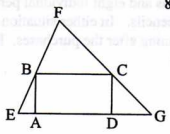
\includegraphics{2007NatTeam.PNG}}

\vskip0.08in
\begin{itemize}
\setlength{\itemindent}{2em}
\item \emph{Solu.:} \hskip0.1in 
\end{itemize}
\vskip1.2in








\clearpage


% 10\sqrt{5}
\item Triangle $MNO$ is an isosceles triangle with $MN=NO=25$ cm. A line segment, drawn from the midpoint of $\overline{MO}$ perpendicular to $\overline{MN}$, intersects $\overline{MN}$ at point $P$ with $NP:PM=4:1$. What is the length of the altitude drawn from point $N$ to $\overline{MO}$? Express your answer in simplest radical form. (2012 State Sprint)

\vskip0.08in
\begin{itemize}
\setlength{\itemindent}{2em}
\item \emph{Solu.:} \hskip0.1in 
\end{itemize}
\vskip1in


% 1624
\item Square $BCFE$ is inscribed in right triangle $AGD$, as shown below. If $AB=28$ units and $CD=58$ units, what is the area of square $BCFE$? (2005 State Sprint)

\centerline{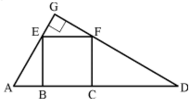
\includegraphics{200529.PNG}}

\vskip0.08in
\begin{itemize}
\setlength{\itemindent}{2em}
\item \emph{Solu.:} \hskip0.1in 
\end{itemize}

\vskip1 in





% 25pi
\item When the diameter of a pizza increases by 2 inches, the area increases by $44\%$. What was the area, in square inches, of the original pizza? Express your answer in terms of $\pi$. (2011 State Sprint)

\vskip0.08in
\begin{itemize}
\setlength{\itemindent}{2em}
\item \emph{Solu.:} \hskip0.1in 
\end{itemize}
\vskip1 in




% 32
\item A right square pyramid with base edges of length $8\sqrt{2}$ units each and slant edges of length 10 units each is cut by a plane that is parallel to its base and 3 units above its base. What is the volume, in cubic units, of the new pyramid that is cut off by this plane? (2009 National Target)

\vskip0.08in
\begin{itemize}
\setlength{\itemindent}{2em}
\item \emph{Solu.:} \hskip0.1in 
\end{itemize}
\vskip1 in







\end{itemize}

\end{itemize}

\clearpage

\centerline{\textbf{\Large{Similarity Problems}}} 
\vskip0.5in

\begin{enumerate}



% 174
\item The surface area of sphere $A$ is $96\%$ more than the surface area of sphere $B$. The volume of sphere $A$ is $r\%$ more than the volume of sphere $B$. What is the value of $r$? Express your answer to the nearest whole number. (2001 Nats Target)

\vskip0.26in

% 98
\item In a trapezoid $ABCD$ with $AB$ parallel to $CD$, the diagonals $AC$ and $BD$ intersect at $E$. If the area of triangle $ABE$ is 50 square units, and the area of triangle $ADE$ is 20 square units, what is the area of trapezoid $ABCD$? (2009 Nats Sprint)

\vskip0.26in

% 120/37
\item Right triangle $ABC$ has one leg of length 6 cm, one leg of length 8 cm, and a right angle at $A$. A square has one side on the hypotenuse of triangle $ABC$ and a vertex on each of the two legs of triangle $ABC$. What is the length of one side of the square? Express your answer as a common fraction. (2007 State Sprint)

\centerline{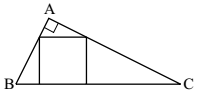
\includegraphics{200730.PNG}}

\vskip0.26in

% 4/21
\item In rectangle $ABCD$, points $E$ and $F$ lie on segments $AB$ and $CD$, respectively, such that $AE=\frac{AB}{3}$ and $CF=\frac{CD}{2}$. Segment $BD$ intersects segment $EF$ at $P$. What fraction of the area of rectangle $ABCD$ lies in triangle $EBP$? Express your answer as a common fraction. (2010 State Sprint)

\vskip0.26in

% 72/13
\item  In the figure below, a 3-inch by 3-inch square adjoins a 10-inch by 10-inch square. What is the area of the region $CDFE$? Express your answer in square inches as a common fraction. (2009 State Target)

\centerline{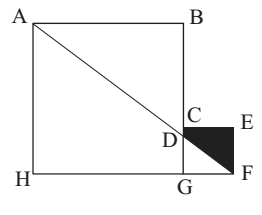
\includegraphics{20097.PNG}}

\vskip0.26in

\clearpage

% 19/37
\item A right circular cone is sliced into four pieces by planes parallel to its base, as shown in the figure. All of these pieces have the same height. What is the ratio of the volume of the second-largest piece to the volume of the largest piece? Express your answer as a common fraction. (2011 State Sprint)

\centerline{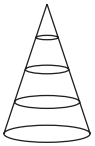
\includegraphics{2011Sprint.PNG}}

\vskip0.26in


% \sqrt{7}
\item In rectangle $ABCD$, $AB=6$ units, the measure of $\angle DBC$ is $30^{\circ}$, $M$ is the midpoint of segment $AD$ and segments $CM$ and $BD$ intersect at $K$. What is the length of segment $MK$? Express your answer in simplest radical form. (2012 MC State Sprint)

\vskip0.26in


% 1 4/5
\item In the figure below, quadrilateral $CDEG$ is a square with $CD=3$, and quadrilateral $BEFH$ is a rectangle. If $BE=5$, how many units is $BH$? Express your answer as a mixed number. (2009 State Team)

\centerline{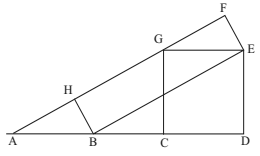
\includegraphics{20099.PNG}}

\vskip0.26in

\centerline{\textit{Super Challenge!}}

\vskip0.2in

% 176
\item A solid right, circular cone has a base radius of 5 meters and a slant height of 10 meters. A top cone will be removed so that the volume of the remaining frustum will be $\frac{1}{3}$ that of the original cone. In square meters, what is the total surface area, including both bases, of the frustum? Express your answer to the nearest whole number. (2014 State Target)

\vskip0.26in

% 126
\item In rectangle $ABCD$, point $M$ is the midpoint of side $BC$, and point $N$ lies on $CD$ such that $DN:NC=1:4$. Segment $BN$ intersects $\overline{AM}$ and $\overline{AC}$ at points $R$ and $S$, respectively. If $NS:SR:RB=x:y:z$, where $x$, $y$, and $z$ are positive integers, what is the minimum possible value of $x+y+z$? (2012 State Sprint)

\vskip0.26in

% 42
\item In square units, what is the largest possible area a rectangle inscribed in a 10-17-21 triangle can have? (2013 State Sprint)

\end{enumerate}


\clearpage

\centerline{\Large{\underline{Mock MATHCOUNTS Target}}}
\vskip 0.7cm

\begin{enumerate}

% 18/5
\item The sum of the first five terms of an arithmetic sequence is 90 less than the sum of the next five terms. What is the absolute difference between two consecutive terms of this sequence? Express your answer as a common fraction. (2016 Chapter Target)

\vskip 7.5cm

\hskip 12cm
\fbox{
	\begin{minipage}{1in}
		\hfill \vspace{0.6in}
	\end{minipage}
	}
	\vskip0.1in
\

\

\

% 81
\item In trapezoid $ABCD$ segments $AB$ and $CD$ are parallel. Point $P$ is the intersection of diagonals $AC$ and $BD$. The area of $\triangle PAB$ is 16 square units, and the area of $\triangle PCD$ is 25 square units. What is the area of trapezoid $ABCD$? (2012 State Sprint)



\vskip5.5cm
\hskip 12cm
\fbox{
	\begin{minipage}{1in}
		\hfill \vspace{0.6in}
	\end{minipage}
	}
	\vskip0.1in



\clearpage


\centerline{\Large{\underline{Mock MATHCOUNTS Target}}}
\vskip 0.7cm



% 24
\item On October 12, to celebrate National Farmer's Day, Farmer Michael gifts Farmer Sujay and Farmer Isaac each with 150 yards of chicken wire. Farmer Sujay and Farmer Isaac each use all 150 yards of wire to make a chicken coop in the shape of a regular polygon. However, the length of each side of Sujay's chicken coop is 30 yards more than the length of each side of Isaac's. If $m$ is the number of sides in Sujay's coop and $n$ is the number of sides in Isaac's, find $m+n$.

\vskip 7.5cm

\hskip 12cm
\fbox{
	\begin{minipage}{1in}
		\hfill \vspace{0.6in}
	\end{minipage}
	}
	\vskip0.1in
\

\

\

% 
\item Binomials



\vskip5.5cm
\hskip 12cm
\fbox{
	\begin{minipage}{1in}
		\hfill \vspace{0.6in}
	\end{minipage}
	}
	\vskip0.1in

\end{enumerate}

\clearpage



%begin Adv Perms
\centerline{\textbf{\Large{Advanced Permutations!}}}

\vskip0.26in

\begin{itemize}

\item \textbf{What is a permutation?} \hskip0.1in 
\vskip0.11in

\begin{itemize} 
\item \emph{To Know:} 
\hskip0.05in Factorials, Symmetry (Rotational, Flippable) 
\end{itemize}
\vskip0.6in



\item \textbf{Examples of Symmetry}
\vskip0.15in




\begin{itemize}
\item \textbf{No Symmetry:} 
\hskip0.05in Find the number of ways to arrange six happy students in a row.  \vskip0.08in
\begin{itemize}
\setlength{\itemindent}{2em}
\item \emph{Solu.:} \hskip0.1in 
\end{itemize}
\vskip0.3in





\item \textbf{Rotational:} \hskip0.05in The same six students are now going to sit around a round table.  How many ways are there to do so?
\vskip0.08in
\begin{itemize}
\setlength{\itemindent}{2em}
\item \emph{Solu:} \hskip0.1in 
\end{itemize}
\vskip0.3in





\item \textbf{Flippable:}  \hskip0.05in 6 round beads are on a bracelet.  How many ways are there to arrange the beads on the bracelet?
\vskip0.08in
\begin{itemize}
\setlength{\itemindent}{2em}
\item \emph{Solu.:} \hskip0.1in 
\vskip0.6in
\end{itemize}
\end{itemize}






\centerline{\emph{\underline{Problems:}}} \vskip0.15in
\begin{enumerate}
\item Lisa is designing a banner for a school play. The banner consists of 4 vertical stripes such that each stripe is a little bit thicker than the one before it. She must choose 4 different colors to paint the stripes out of 9 available colors. In how many ways can she do this?  \emph{(GliyaNet)}
\vskip0.2in
	
\item Tim is designing a banner for a school play. The banner consists of 4 horizontal stripes. He asks Heather to grab 4 differently colored cloth stripes from the supply closet. When Heather arrives at the supply closet she finds that there are cloth stripes of 9 different colors. In how many distinct ways can she choose from among the cloth stripes to help Tim with his banner? (How are problems 1 and 2 different?)  \emph{(GliyaNet)}
\vskip0.2in 


\item A license plate consists of two letters followed by two digits; for example, MP78. Neither the digits nor the letters may be repeated, and neither the letter ``O" nor the digit ``0" may be used. When reading from left to right, the letters must be in alphabetical order and the digits must be in increasing order. How many different license plate combinations are possible? (MATHCOUNTS)


\end{enumerate}  
\vskip0.2in
\newpage











\centerline{\textbf{\Large{More Advanced Permutations}}} \vskip0.05in
\vskip0.33in




\item \textbf{Dealing With Restrictions}
\vskip0.15in

To deal with restrictions, you have to apply multiple combo methods. There are many more restrictions than the ones shown here.

\vskip0.15in


\begin{itemize}
\item \textbf{Arrangement Restrictions:} \hskip0.05in A license plate is made of three different letters of the English alphabet along with three digits.  Find the number of ways to make a license plate given that the digits must all be placed adjacently to each other.
\vskip0.06in
\begin{itemize}
\setlength{\itemindent}{2em}
\item \emph{Solu.:} \hskip0.1in 
\end{itemize}
\vskip0.6 in





\item \textbf{Circular Restrictions} \hskip0.05in Representatives from eight lands are sitting around a circular table. The Flurgaburbur representative has 6 dinner rolls. The representatives have agreed that everyone will have exactly one more or one less dinner roll than each of their neighbors. How many different ways are there to give the representatives rolls such that the restriction is met? (AoPS)\vskip0.08in
\begin{itemize}
\setlength{\itemindent}{2em}
\item \emph{Solu:} \hskip0.1in 
\end{itemize}
\vskip0.6 in






\item \textbf{Groups of Groups:} \hskip0.05in Six students are being grouped into three pairs.  In how many ways can this be done?
\vskip0.08in
\begin{itemize}
\setlength{\itemindent}{2em}
\item \emph{Solu.:} \hskip0.1in 
\end{itemize}
\vskip0.6in
\end{itemize}
\end{itemize}
\vskip0.15 in





\centerline{\emph{\underline{Problems:}}} \vskip0.15in
\begin{enumerate}


% 560
\item Define a good word as a sequence of letters that consists only of the letters A, B, and C � some of these letters may not appear in the sequence � and in which A is never immediately followed by B, B is never immediately followed by C, and C is never immediately followed by A. How many seven-letter good words are there? \emph{(AIME)} 
\vskip0.2in

% 192
\item In a shooting match, eight clay targets are arranged in two hanging columns of three targets each and one column of two targets. A marksman is to break all the targets according to the following rules: \newline
(1) The marksman first chooses a column from which a target is to be broken.\newline
(2) The marksman must then break the lowest remaining target in the chosen column. \newline
If the rules are followed, in how many different orders can the eight targets be broken? \emph{(AIME)}
\vskip0.2in


% 192
\item Nine students named M, A, T, H, C, O, U, N, and S, are deciding how to sit around a circular table.  M says he must sit next to his girlfriend N, but O and U are arch rivals and refuse to sit next to each other.  In how many ways can the students do so?
\vskip0.2in


\end{enumerate}

\clearpage


\centerline{\textbf{\Large{Combinatoricaliti-... Say What?}}} \vskip0.1in
\centerline{\textbf{\texttt{Combinatorics}}}

\vskip0.33in


\begin{enumerate}

% 
% Answer: 
\item In how many ways can a starting lineup (a committee of five) be formed from the 12 members of a basketball team? Assume that the lineup is the same, even if the positions played by the team members are shuffled around. 
\vskip0.26in




%
% Answer: 
\item On Old Mackonald's farm, there are 4 Chinese cows, 5 German cows, 7 Mexican cows, and 5 pieces of asparagus. If Old Mackonald wants to select a group of 2 German cows, 3 Mexican cows, and 2 pieces of asparagus, how many ways are there for him to do so?

\vskip0.26in



% 
% Answer: 
\item In how many ways can a committee of four senators be chosen if no two senators can be from the same state? 
 
\vskip0.26in




% 
% Answer: 
\item Ten points are marked on a circle. How many distinct convex polygons of three or more sides can be 
drawn using some (or all) of the ten points as vertices? (AIME) 

\vskip0.26in



% 
% Answer: 
\item Each of a set of eight parallel lines in a plane intersects with each line from a different set of six parallel lines. Find the total number of parallelograms formed by these intersections. 

\vskip0.26in




% 
% Answer: 
\item A permutation $(a_1, a_2, a_3, a_4, a_5)$ of $(1, 2, 3, 4, 5)$ is ``heavy-tailed" if $a_1 + a_2 < a4 + a_5$. What is the number of ``heavy-tailed" permutations? (AMC 12) 

\vskip0.26in




%
% Answer: 
\item Find the maximum number of points of intersection between twelve lines in a plane. (What if one pair of them is parallel?)


\vskip0.9in

\newpage

\centerline{\emph{Zee Extrah Challenzhe Problehms!}}
\vskip0.33in
%
% Answer: 70
\item What is the maximum possible number of intersection points of diagonals inside a convex octagon? (AoPS)

\vskip0.26in



%
% Answer: 
\item A spider has one sock and one shoe for each of its eight legs. On each leg the sock must be put on before the shoe. In how many different orders can the spider put on its socks and shoes? (AMC 10) 

\vskip0.26in


%
% Answer: 
\item Let $(a_1,a_2,a_3,...,a_12)$ be a permutation of $(1,2,3, ..., 12)$ for which $a_1 >a_2 >a_3 >a_4 >a_5 >a_6$ and $a_6 <a_7 <a_8 <a_9 <a_{10} <a_{11} <a_{12}$. 
An example of such a permutation is $(6, 5, 4, 3, 2, 1, 7, 8, 9, 10, 11, 12)$. Find the number of such permutations. (AIME) 

\vskip0.26in



%
% Answer: 
\item Ninety-four bricks, each measuring 4"$\times$ 10"$\times$ 19", are to be stacked one on top of another to form a tower 94 bricks tall. Each brick can be oriented so it contributes 4" or 10" or 19" to the total height of the tower. How many different tower heights can be achieved using all 94 of the bricks? (AIME) 
\vskip0.26in







\end{enumerate}

\clearpage

\centerline{\textbf{\Large{Modular Arithmetic}}}
\vskip0.1in
\centerline{\textit{it's just arithmetic...sort of}}
\vskip0.33in

Modular arithmetic, also called mods, is a branch of mathematics used to solve for remainders when an integer is divided by another integer. 
\vskip0.17in


\indent \indent  \indent $-$ \emph{Definition:}  $m\equiv n \bmod{p}$ is equivalent to $\frac{m-n}{p}\in N$. In other words, $m-n$ is a multiple of $p$. \\

\vskip-0.18in \hskip1.28in For example: $53\equiv 3\bmod{5}$. Note that the symbol $``\equiv"$ is used, not $``="$. \\ \vskip-0.18in \hskip1.28in Also, note that 5 is what we call our \textbf{modulus}.
\\ \vskip-0.18in \hskip1.28in
In terms of the Division Theorem, if $x=pq+r$, then $x\equiv r \bmod p$ (very important)


\vskip0.42in

\textbf{The Basics}: Mods  have their own system of arithmetic (hence, modular arithmetic)
\vskip0.05in
\begin{itemize}[leftmargin=0.6in]
\item $a+b\pmod{n}\equiv a\pmod{n}+b\pmod{n}$
\vskip0.05in
\item $a\times b\pmod{n}\equiv a\pmod{n}\times b\pmod{n}$
\vskip0.05in
\item Subtraction exists too, with the idea of negative mods 
\vskip0.05in
\item Division sort of exists. But it's more complicated.
\end{itemize}

\vskip.2in

\begin{itemize}


\renewcommand{\labelitemi}{$\bullet$ \hskip0.04in}
\renewcommand{\labelitemii}{$\cdot$}
\renewcommand{\labelitemiii}{$\diamond$}
\renewcommand{\labelitemiv}{$\ast$}


\item \textbf{Find 109 mod 9}. 
\vskip0.08in
\begin{itemize} 
\item We start by finding the smallest multiple of 9 less than 109.  We know 90 is a multiple of 9, so we add 18, which is another multiple of 9, to get 108, another multiple of 9. Thus, $109 \equiv 109-108\equiv 1\bmod{9}$.
\end{itemize}


\vskip0.2in




\item \textbf{Find $-$2 mod 8.} 

\vskip0.08in
\begin{itemize}
\item This problem may look a bit strange at first, but thinking outside the box would definitely help. Let us subtract a negative multiple of 8:  $-2 \equiv -2-(-8) \equiv 6 \bmod{8}$.  Now we see that $-2\equiv 6\bmod{8}$.
\end{itemize}


\vskip0.2in


\item \textbf{Find the last digit of 8$\times$6$\times$7$\times$2$\times$13$\times$19.} 

\vskip0.08in
\begin{itemize}
\item The last digit of an integer is the remainder when the integer is divided by 10.  Let's rewrite each of the integers in mod 10.   This still looks rather messy, so we simplify by multiplying out the negatives.  Observing the problem above, we discover that
 $8\times 6\times 7\times 2\times 3\times 9 \equiv (-2)\times(-4)\times (-3) \times 2\times 3\times (-1) \equiv 8\times 9\times 2 \equiv 4 \bmod{10}$.
\end{itemize}


\vskip0.2in

\item \textbf{Find the remainder when $3^{523}$ is divided by 13.} 
\vskip0.08in
\begin{itemize}
\item We may just list powers until we find a pattern. 

Note that $3^1\equiv 3\pmod{13}$, $3^2\equiv 9\pmod{13}$, $3^3\equiv 1\pmod{13}$, and we can stop here. 

Then $3^{3k}\equiv 1\pmod{13}$ so $3^{523}\equiv 3^{522}\times 3\pmod{13}\equiv 3\pmod{13}$

\end{itemize}

\vskip0.2in

\item \textbf{Find \emph{n} such that \emph{5n} $\equiv$ 2 mod 7.} 

\vskip0.08in
\begin{itemize}
\item Since mods are only defined by integers, we conclude that $n\ne \frac{2}{5}$.  We can add 7 to the right side, since $5n\equiv 2+7m \bmod{7}$, or $a\equiv b+kp\bmod{p}$, where $a$, $b$, $k$, and $p$ are integers.  Now, we get $5n\equiv 9\bmod{7}$.  Did that help much? It's debatable. (In other words, no.) Let's add more 7�s.  9 + 7 = 16.  16 + 7 = 23.  23 + 7 = 30.  Indeed, 30 is a multiple of 5.  So we have $n \equiv 6\bmod{7}$.
\end{itemize}

\item \textbf{Find all $n$ such that 6a+5$\equiv$ 3 mod 4}

\vskip0.08in
\begin{itemize}
\item We can simplify it like we would a normal equation.

\begin{align*}
6a+5 &\equiv 3\bmod{4}\\
6a &\equiv 2\bmod{4} \\
2a & \equiv 2\bmod{4}
\end{align*}

However, we have to be a little careful in finishing this off, we can't just say $a\equiv 1\bmod{4}$.

Note that $2a \equiv 2\bmod{4}$ is equivalent to saying $2a=4b+2$ for some $b$.

Then $a=2b+1$, or \fbox{$a\equiv 1\bmod{2}$}, which indeed works.
\end{itemize}
\vskip0.4in

\textbf{\large{Linear Congruences}}

\vskip0.2in

Just as we have systems of equations in algebra, we have \textit{linear congruences} in modular arithmetic.
\vskip0.05in
Essentially, we are given two modular congruences and told to combine them into one.

\vskip0.1in
\item \textbf{Describe all integers $n$ that have a remainder of 0 when divided by 4 and a remainder of 9 when divided by 11} 
\vskip0.08in
\begin{itemize}
\item We may write the conditions as 
\begin{align*}
n &\equiv 0\bmod{4} \\
n &\equiv 9\bmod{11}
\end{align*}

But saying $n\equiv 9 \bmod{11}$ is the same as saying $n=11a+9$ for some integer $a$.

We use this simple observation by plugging back into the other congruence to get

\begin{align*}
11a+9 & \equiv 0 \bmod{4} \\
3a+1 & \equiv 0 \bmod{4} \\
3a & \equiv 3\bmod{4} \\
a &\equiv 1 \bmod{4}
\end{align*}

Now we rewrite this in division form again and write $a=4b+1$ for some $a$. 

But originally, we wanted to describe $n$. We had $n=11a+9$, so plugging in $a=4b+1$, we get $n=44b+20$, or \fbox{$n\equiv 20\bmod{44}$}.

\vskip0.2in

\textit{Note}: This is indeed all solutions $n$. However, there are a couple of important details too technical to explain here. The technique we used above will always work if you use it correctly though.

\end{itemize}

\vskip0.2in

% 39
\item \textbf{When a positive integer is divided by 7, the remainder is 4. When the same integer is divided by 9, the remainder is 3. What is the smallest possible value of this integer?} (2008 State Sprint)
\vskip0.08in
\begin{itemize}
\setlength{\itemindent}{2em}
\item \emph{Solu.:} \hskip0.1in 
\end{itemize}
\vskip0.4 in


%
\item\textbf{Find the smallest positive integer n such that n$\equiv$ 4 mod 7, and n$\equiv$ 5 mod 8.}
\vskip0.08in
\begin{itemize}
\setlength{\itemindent}{2em}
\item \emph{Solu.:} \hskip0.1in 
\end{itemize}
\vskip0.4 in

\end{itemize}

\clearpage

\centerline{\textbf{\Large{Applications of Mods}}}

\vskip0.4in

\textbf{\large{Divisibility Rules}}
\vskip0.2in
Have you ever wondered why the divisibility rules work?

\vskip0.1in
\begin{itemize}
\item \textbf{Prove the divisibility rule for 3.}
\vskip0.1in
\begin{itemize}
\item We actually claim that a number is always congruent to the sum of its digits mod 3.

Suppose we have some number $\overline{a_1a_2a_3a_4a_5}$.

We may expand this as $\overline{a_1a_2a_3a_4a_5}=10^4\cdot a_1+10^3\cdot a_2+10^2\cdot a_3+10\cdot a_4+a_5$

Then 

\begin{align*}
10^4\cdot a_1+10^3\cdot a_2+10^2\cdot a_3+10\cdot a_4+a_5 &\equiv 1^4\cdot a_1+1^3\cdot a_2+1^2\cdot a_3+1\cdot a_4+a_5 \pmod{3} \\
&\equiv a_1+a_2+a_3+a_4+a_5 \pmod{3}
\end{align*}

\end{itemize}

\item \textbf{Divisibility rule for 11: Check if the alternating sum of the digits is divisible by 11}
\vskip0.08in
\begin{itemize}
\setlength{\itemindent}{2em}
\item \emph{Solu.:} \hskip0.1in 
\end{itemize}
\vskip0.8 in
\end{itemize}
\vskip0.5in

\textbf{\large{Base Arithmetic}}

\vskip0.2in

Mods are helpful with base number problems for an obvious reason.

\vskip0.1in

\begin{itemize}
\item \textbf{What is the last digit in the base 9 representation of $5^{45}$?}

\vskip0.08in
\begin{itemize}
\setlength{\itemindent}{2em}
\item \emph{Solu.:} \hskip0.1in 
\end{itemize}
\vskip0.8 in

\end{itemize}

\textbf{\large{More on Powers}}

\vskip0.2in

Exponent problems can get more complicated, but deal with it the same way.
\vskip0.1in
\begin{itemize}
\item \textbf{Albus claims that $21^{21^{21}}$ has a remainder of 5 when divided by 12, and Aberforth claims that it has a remainder of 5 when divided by 13. Who is correct? Is either of them right?}
\vskip0.08in
\begin{itemize}
\setlength{\itemindent}{2em}
\item \emph{Solu.:} \hskip0.1in 
\end{itemize}
\vskip0.8 in

\end{itemize}



\clearpage

\centerline{\textbf{\Large{Moderately Difficult Mods}}} \vskip0.1in
\centerline{\texttt{Advanced Modular Arithmetic}}
\vskip0.33in

\vskip0.15in

\begin{enumerate}

% Saturday
\item The War of $1812$ started with a declaration of war on Thursday, June $18$, $1812$. The peace treaty to end the war was signed $919$ days later, on December $24$, $1814$. On what day of the week was the treaty signed? (2016 AMC 12B)

\vskip0.26in

% 3
\item The Fibonacci sequence is the sequence $1$, $1$, $2$, $3$, \ldots where each term is the sum of the previous two terms. What is the remainder when the 100th term of the sequence is divided by $4$? (2005 State Sprint)

\vskip0.26in

% 3
\item The base-10 numbers 217 and 45 are multiplied. The product is then written in base-6. What is the units digit of the base-6 representation? (2001 National Sprint)

\vskip0.26in

% 109
\item Find the remainder when $9 \times 99 \times 999 \times \cdots \times \underbrace{99\cdots9}_{\text{999 9's}}$ is divided by $1000$. (2010 AIME I)

\vskip0.26in

% 
% Answer: 
\item What is the remainder when $17^{17}+18^{18}+19^{19}$ is divided by 7?
\vskip0.26in



% 7
\item Find the remainder when the sum of the squares of the first 2014 integers are divided by 8.
\vskip.26in


% 2^{1005}
\item What is the greatest power of 2 that is a factor of $10^{1002}-4^{501}$? (2014 AMC 10B)

\vskip0.26in


% 4
\item The 9-digit number $abb,aba,ba3$ is a multiple of $99$ for some pair of digits $a$ and $b$. What is $b-a$? (2002 National Team)
\vskip0.26in



% 935
\item An integer $X$ is a multiple of 17, is one less than a multiple of 8, and is less than 1000. What is the largest possible value of $X$? (2009 State Sprint)

\vskip0.26in

% 479
\item The arithmetic progressions $\{ 2, 5, 8, 11, \ldots\}$ and $\{3, 10, 17, 24, \ldots\}$ have some common values. What is the largest value less than $500$ that they have in common?

\vskip0.26in

% 1/4
\item Two random integers $a$ and $b$ are independently chosen, with replacement, from $1$ to $1000$ inclusive. What is the probability that both $2^a+2^b$ and $3^a+3^b$ are multiples of $5$? Express your answer as a common fraction. (2014 National Sprint)

\vskip0.26in


% 
% Answer: 865
\item Yuti is writing down all the integers from 1 to 2015, inclusive, on potatoes, to give to Emily as a birthday present. However, to make it even more amazing, she decides that she doesn't want any pair of these numbers to sum to a multiple of 7. What is the largest possible number of integers that she can keep to satisfy this condition? 

\end{enumerate}

\clearpage








\centerline{\textbf{\Large{Powerful Powers Techniques}}}
\vskip0.4in

There are actually some more ways we can compute powers with mods that make it even easier.

\vskip0.1in

\textbf{Fermat's Little Theorem}
\vskip0.1in
\begin{itemize}
\item For every integer $a$ and prime $p$, $a^p\equiv a\bmod{p}$ 
\vskip0.05in
\item Alternatively, if $p$ does not divide $a$, $a^{p-1}\equiv 1\bmod{p}$
\end{itemize}

\vskip0.2in
\textbf{Euler's Totient Theorem}
\vskip0.1in
\begin{itemize}
\item A more general version of Fermat's theorem
\vskip0.05in
\item For relatively prime integers $a$ and $n$, $a^{\phi(n)}\equiv 1\bmod{n}$
\item $\phi(n)$ denotes the number of positive integers less than $n$ relatively prime to $n$\vskip0.05in
\begin{itemize}
\item If $n=p_1^{r_1}\cdot p_2^{r_2}\cdots p_k^{r_k}$, then $\phi(n)=n\cdot(1-\frac{1}{p_1})\cdot(1-\frac{1}{p_2})\cdots(1-\frac{1}{p_k})$
\vskip0.05in
\item For example, $\phi(20)=20\cdot\frac{1}{2}\cdot\frac{4}{5}=4$ and $\phi(120)=120\cdot\frac{1}{2}\cdot\frac{2}{3}\cdot\frac{4}{5}=32$
\end{itemize}
\vskip0.05in
\item The condition on this one is actually important
\end{itemize}

\vskip0.4in

\textbf{Using our new tricks}
\vskip0.1in
\begin{itemize}
\item What is the remainder when $17^{17}+18^{18}+19^{19}$ is divided by 7?
\vskip0.1in
\begin{itemize}
\item Revisiting this problem with our new tricks, it gets even shorter.

First we do the simple reduction mod 7 to get
\vskip-0.1in
$$17^{17}+18^{18}+19^{19}\equiv 3^{17}+4^{18}+5^{19}\pmod{7}$$

Now since $p$ is prime, $a^6\equiv 1\bmod 7$ as long as $a$ is not $0\bmod{7}$, so

\begin{align*}
3^{17}+4^{18}+5^{19} &\equiv 3^5+1+5^1\pmod{7} \\
&\equiv 243+1+5\pmod{7} \\
&\equiv 4\pmod{7}
\end{align*}

\end{itemize}

\vskip0.2in
% 16
\item What is the remainder when $2014^{2014}$ is divided by 100?

\vskip0.1in

\begin{itemize}
\item First we reduce to $14^{2014}\bmod 100$, and then...we get stuck.
\vskip0.05in
This one's not as nice because $gcd(2014, 100)\neq 1$ so we can't just straight out apply Euler's Theorem. 
\vskip0.05in
The crucial step is that instead of taking it mod 100 directly, we take $14^{2014}\bmod 4$ and mod 25 (we have to split it into prime powers for this to work) and then try to combine these later.
\vskip0.05in
Clearly $14^{2014}\equiv 0\bmod{4}$.
\vskip0.05in
Now we want $14^{2014}\bmod{25}$. This time, we can apply Euler's theorem to note that
\vskip0.05in
\centerline{$14^{\phi(25)}\equiv 14^{20}\equiv 1\bmod{25}$, so $14^{2014}\equiv 14^{14}\bmod{25}$.} 

\vskip0.05in
This is still gross, but much easier. To minimize computation, we only compute exponents of 2.

\clearpage
$14^1\equiv 14\equiv -11\bmod{25}$

$14^2\equiv (-11)^2\equiv 121\equiv -4\bmod{25}$

$14^4\equiv (-4)^2\equiv 16\bmod{25}$

$14^8\equiv (-9)^2\equiv 6\bmod{25}$

Finally, $14^{14}\equiv 14^8\cdot 14^4\cdot 14^2\equiv 6\cdot 16\cdot (-4)\equiv 16\bmod{25}$

Now we're almost done. We know that our desired number is $0\bmod{4}$ and $16\bmod{25}$. If we work out the linear congruence, we get that the number is \fbox{$16\bmod{100}$}


\end{itemize}
\end{itemize}

\vskip0.4in

One other note: there is one other technique to be aware of when dealing with powers. See the following:
\vskip0.1in

\begin{itemize}
\item Find the last two digits of $9^{2016}$.

\begin{itemize}
\item We could do the trick with splitting mod 100 into mod 4 and mod 25, but that would be very tedious.
\vskip0.05in
The crucial observation is that we want $9^{2016}\bmod{100}$ and $9$ is just one less than 10. 
\vskip0.05in
Then the clever idea is to write $9^{2016}=(10-1)^{2016}$ then expand with binomial theorem.

Try and work out the details on your own, but you should get 
\vskip-0.1in
$$9^{2016}\equiv 2016\cdot 10\cdot (-1)^{2015}+1\equiv \fbox{41}\bmod{100}$$
\end{itemize}


\vskip0.5in

\end{itemize}

\textbf{Try it out!}
\vskip0.2in

\begin{enumerate}
% 1, 13, 40
\item Compute the following expressions:

\begin{itemize}
\item $5^{244} \bmod {13}$
\item $13^{441} \bmod {25}$ 
\item $10^{342}\bmod{65}$
\end{itemize}
\vskip0.26in

% 8
\item When the expression $(2^1)(2^2)\ldots (2^{99})(2^{100})$ is written as an integer, what is the product of the tens digit and the ones digit? (2007 State Target)
\vskip0.26in

% 7
\item How many zeroes occur at the end of the number $1999^6+6\cdot 1999+5$? (Mandelbrot)
\vskip0.26in

% 35
\item Let $a_n$ equal $6^{n}+8^{n}$. Determine the remainder upon dividing $a_ {83}$ by $49$. (1983 AIME)

\end{enumerate}

\clearpage

\centerline{\textbf{\Large{More Factorizations!}}} \vskip0.1in
\centerline{\ldots with numbers this time!}
\vskip0.33in

\begin{itemize}

\item \textbf{Nice Identities}
\vskip0.17in
\begin{itemize}
\item\textbf{Let $n=p_1^{r_1}\cdot p_2^{r_2}\cdots p_i^{r_i}$ where the $p_i$ are all primes.}
\vskip0.15in
\begin{itemize}
\item Every number has a unique prime factorization (so the $p_i$'s and $r_i$'s are unique to each $n$)
\vskip0.05in
\item The number of factors of $n$, call it $\# (n)$, is $(r_1+1)(r_2+1)\cdots (r_i+1)$. 
\vskip0.05in
\item The product of factors of $n$ is $n^{\frac{\#(n)}{2}}$
\vskip0.05in
\item The sum of factors of $n$ is 
\vskip-0.15in
$$(1+p_1+\ldots +p_1^{r_1})(1+p_2+\ldots +p_2^{r_2})\cdots (1+p_i+\ldots+p_i^{r_i})$$ 
\vskip0.05in
or more concisely, 

$$\left(\frac{p_1^{r_1+1}-1}{p_1-1}\right)\left(\frac{p_2^{r_2+1}-1}{p_2-1}\right)\cdots \left(\frac{p_i^{r_i+1}-1}{p_i-1}\right)$$
\end{itemize}
\end{itemize}
\vskip0.4in
\item \textbf{Problems!}
\vskip0.2in

\begin{itemize}





\item When all of the factors of $90$ are multiplied together, the product can be expressed as $90^k$. What is the value of $k$? (2011 National Target)
\vskip0.08in
\begin{itemize} 
\setlength{\itemindent}{2em}
\item \emph{Solu.:} \hskip0.1in 
\end{itemize}
\vskip1.1 in





\item The first term of an arithmetic sequence is $1$, another term of the sequence is $91$ and all of the terms of the sequence are integers. How many distinct arithmetic sequences meet these three conditions? (2008 State Sprint)

\vskip0.08in
\begin{itemize}
\setlength{\itemindent}{2em}
\item \emph{Solu:} \hskip0.1in 
\end{itemize}
\vskip1.1 in


% 60
\item Given that $n>1$, what is the smallest positive integer $n$ whose divisors have a product of $n^6$? (2009 National Target)
\vskip0.08in
\begin{itemize}
\setlength{\itemindent}{2em}
\item \emph{Solu.:} \hskip0.1in 
\end{itemize}
\vskip1.1 in

% 2
\item Find the sum of the reciprocals of the positive divisors of 496. (2007 VHHS)
\vskip0.08in
\begin{itemize}
\setlength{\itemindent}{2em}
\item \emph{Solu.:} \hskip0.1in 
\end{itemize}
\vskip1.1 in


% 144
\item Cindy wishes to arrange her coins into $X$ piles, each consisting of the same number of coins, $Y$. Each pile will have more than one coin and no pile will have all the coins. If there are 13 possible values for $Y$ given all of the restrictions, what is the smallest number of coins she could have? (2009 State Target)
\vskip0.08in
\begin{itemize}
\setlength{\itemindent}{2em}
\item \emph{Solu.:} \hskip0.1in 
\end{itemize}
\vskip1.1 in

% 8
\item Find the least positive integer $n$ such that no matter how $10^{n}$ is expressed as the product of any two positive integers, at least one of these two integers contains the digit $0$. (2000 AIME I)
\vskip0.08in
\begin{itemize}
\setlength{\itemindent}{2em}
\item \emph{Solu.:} \hskip0.1in 
\end{itemize}
\vskip1.1 in


\end{itemize}




\end{itemize}

\clearpage

\centerline{\Large{\textbf{Still More Factorizations}}} \vskip0.6in


\begin{enumerate}



% 722
\item What is the sum of the three numbers less than 1000 that have exactly five positive integer divisors? (2000 National Sprint)
\vskip0.52in

% 14.8
\item A teenager is someone who is 13, 14, 15, 16, 17, 18, or 19 years old. The product of the ages of a particular group of teenagers is 705,600. What is the mean of their ages? Express your answer as a decimal to the nearest tenth. (2007 State Target)

\vskip0.52in

% 
% 240
\item Emma plays with her square unit tiles by arranging all of them into different shaped rectangular figures. (For example, a 5 by 7 rectangle would use 35 tiles and would be considered the same rectangle as a 7 by 5 rectangle). Emma can form exactly ten different such rectangular figures that each use all of her tiles. What is the least number of tiles Emma could have? (2006 State Team)

\vskip0.52in



% 
% 24
\item The product of all the positive factors of $6^3$ can be written in the form $6^M$, for some positive integer $M$. What is the value of $M$? (2010 National Target)
\vskip0.52in


% 281
\item The integer 12 has five one-digit factors, 20 has four one-digit factors, and together 12 and 20 have nine one-digit factors (some of which are repeats.) What is the total number of one-digit factors for all of the integers from $1$ to $100$, inclusive? (2010 State Target)
\vskip0.52in


% 634
\item Let $m/n$, in lowest terms, be the probability that a randomly chosen positive divisor of $10^{99}$ is an integer multiple of $10^{88}$. Find $m+n$. (1988 AIME)
\vskip0.52in

% 432
\item Let $n$ be the smallest positive integer that is a multiple of 75 and has exactly 75 positive integral divisors, including 1 and itself. Find $n/75$. (1990 AIME)
\vskip0.52in

% 180
\item What is the smallest positive integer with six positive odd integer divisors and twelve positive even integer divisors? (2000 AIME II)




\vskip0.52in



\end{enumerate}

\clearpage

\centerline{\Large{\textbf{Binomial Theorem}}}
\vskip0.1in
\centerline{And Relating Concepts}
\vskip0.33in

\begin{itemize}

\item \textbf{Review}
\vskip0.2in
\begin{itemize}
\item What is a monomial?
\item What is a binomial?
\item Expand $(a+b)^2$ 
\vskip0.08in
\begin{itemize}
\setlength{\itemindent}{2em}
\item \emph{Solu.:} \hskip0.1in 
\end{itemize}
\vskip0.65in
\item Expand $(x+y)^3$
\vskip0.08in
\begin{itemize}
\setlength{\itemindent}{2em}
\item \emph{Solu.:} \hskip0.1in 
\end{itemize}
\vskip0.65in
\item Theorem allows you to predict coefficients of terms in expansions

\end{itemize}
\vskip0.4in
\item\textbf{Formula and Derivation}
\vskip0.2in
\begin{itemize}
\centerline{\Large{$(a+b)^n = \sum_{k=0}^{n}\binom{n}{k}a^{n-k}b^k$}} \vskip0.1in
\item When looking for one term, ignore the summation symbol
\item Any binomial to some power can be written out as $n$ binomials multiplied out
\item The coefficient is dependent on how many times you can make that specific like term
\item You need to "choose" enough $a$'s and $b$'s

\end{itemize}

\end{itemize}



\end{document}